\section{O1 results}

Advanced LIGO's first observing run lasted from September 12, 2015 - 
January 19, 2016.  

We found GW150914!

\begin{figure}[ht!]
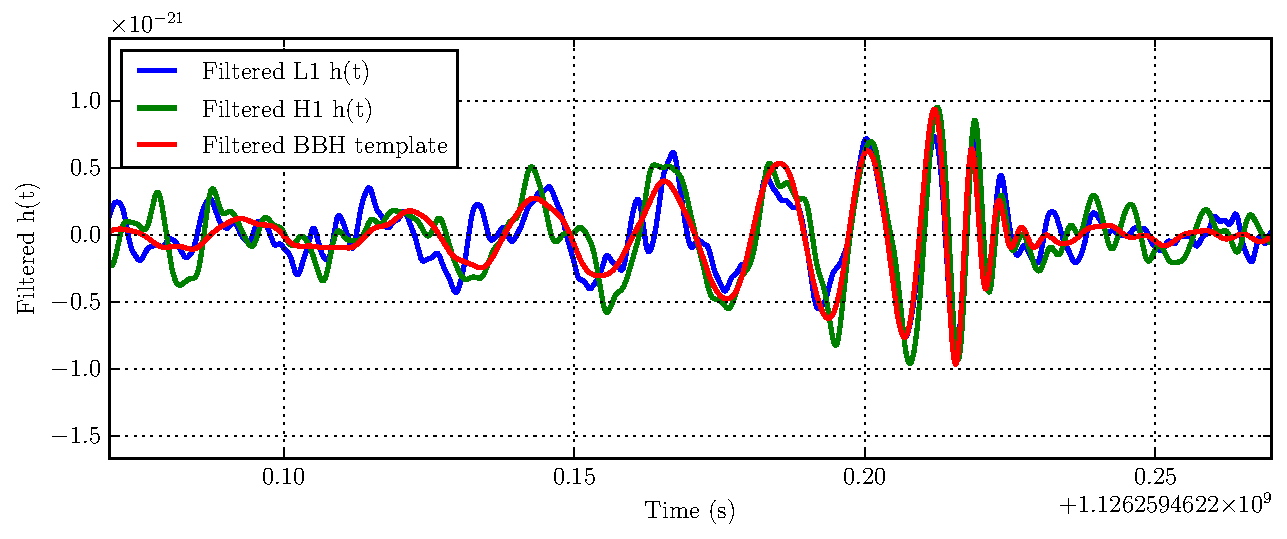
\includegraphics[width=\textwidth]{figures/O1/GW150914-timeseries}
\caption[GW150914 timeseries]{Time-domain representation of L1 %
        gravitational wave strain at the time of GW150914. The blue %
        curve is strain, zero-phase bandpass filtered to isolate the %
        frequencies that contain signal. The red curve is a CBC waveform %
        generated using the best estimated parameters. The CBC waveform %
        has been filtered in the same way as the strain curve.}
\end{figure}\label{fig:GW150914}

We also found GW151226!

LVT151012 was interesting.

\section{PyCBC results}

How significant was GW150914? Figure \ref{fig:pycbc-hist-gw150914} can 
tell us!

\begin{figure}[ht!]%
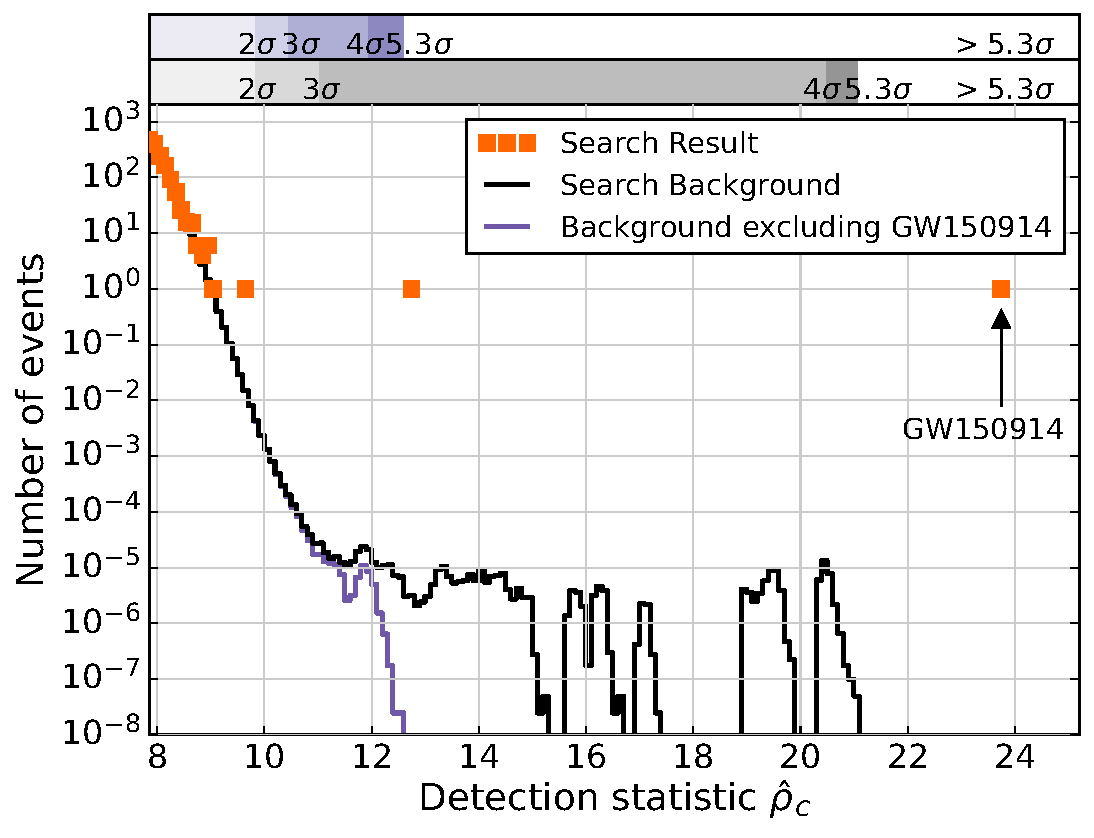
\includegraphics[width=\textwidth]{figures/O1/pycbc_hist_GW150914}
\caption[PyCBC result histograms for GW150914]{Histograms of PyCBC results for GW150914}
\end{figure}\label{fig:pycbc-hist-gw150914}

How significant was GW151226? We have to remove GW150914 to find out. 
Then Figure \ref{fig:pycbc-hist-gw151226} can tell us!

\begin{figure}[ht!]%
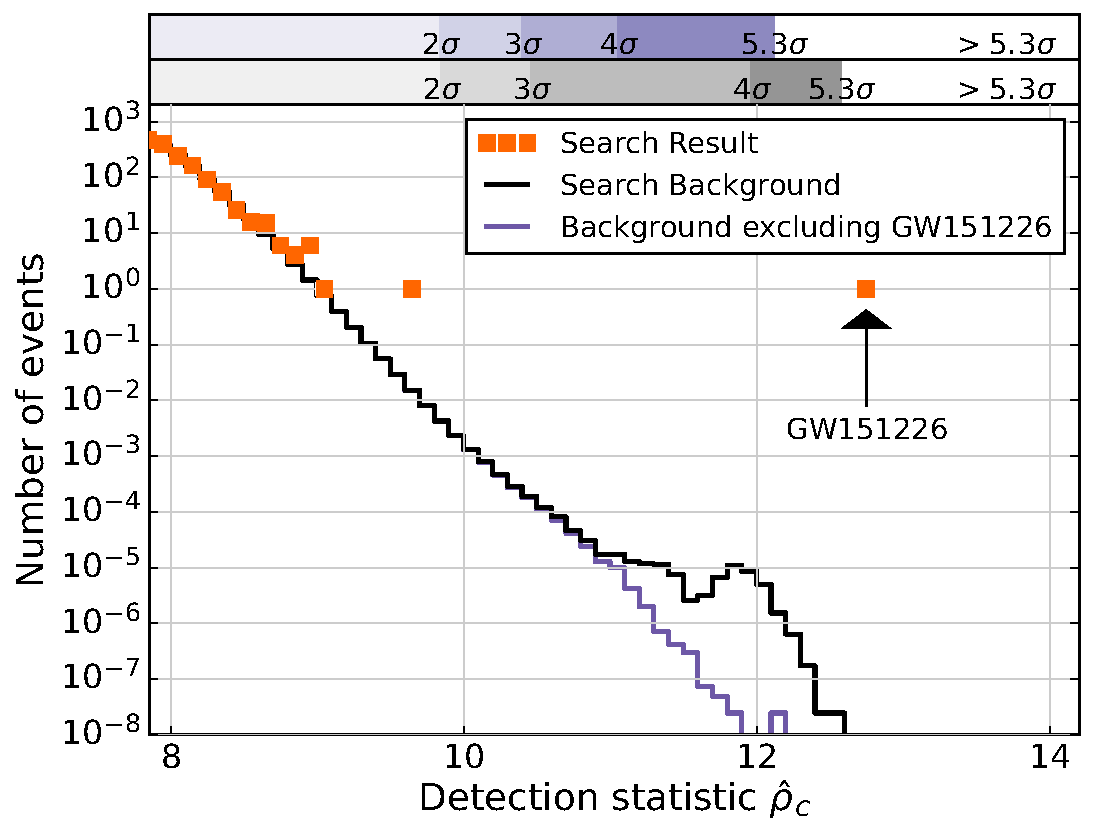
\includegraphics[width=\textwidth]{figures/O1/pycbc_hist_GW151226}
\caption[PyCBC result histograms for GW151226]{Histograms of PyCBC results for GW151226}
\end{figure}\label{fig:pycbc-hist-gw151226}

